\subsection{Base de Imagens e Visualização} \label{metodoBaseImg}

Para a geração das imagens HDR nos métodos das próximas subseções, será utilizada a base de imagens LDR aqui apresentada. Essa base de dados consiste num conjunto de cenas, cada uma possuindo regiões bem iluminadas e regiões pouco iluminadas. Cada cena foi registrada por um conjunto de imagens LDR, que diferem apenas em tempo de exposição, e cada imagem busca registrar uma faixa de iluminação específica da cena. Com isso visa-se verificar a eficiência de cada método em gerar imagens HDR dessas cenas.

É importante salientar que, apesar de pouco, o movimento entre a captura das imagens LDR de cada cena da base de dados existe. Esse foi um fator limitante neste trabalho, devido aos equipamentos disponíveis para uso. Outro fator limitante devido ao equipamento utilizado foi o uso de imagens no formato JPG, que possui compressão com perda de informações.

\subsubsection{Cena da Didática} \label{cenaDidatica}

\begin{figure}[H]
  \subfloat[Tempo de exposição de $0.002s$.]
  {
    \includegraphics[height=4cm]{CenaDidatica/1}
    \label{figBaseDidaticas1}
  }
  \quad %espaco separador
  \subfloat[Tempo de exposição de $0.005s$.]
  {
    \includegraphics[height=4cm]{CenaDidatica/2}
    \label{figBaseDidaticas2}
  }
  \quad %espaco separador
  \subfloat[Tempo de exposição de $0.0167s$.]
  {
    \includegraphics[height=4cm]{CenaDidatica/3}
    \label{figBaseDidaticas3}
  }
  \quad %espaco separador
  \subfloat[Tempo de exposição de $0.04s$.]
  {
    \includegraphics[height=4cm]{CenaDidatica/4}
    \label{figBaseDidaticas4}
  }
  \quad %espaco separador
  \subfloat[Tempo de exposição de $0.067s$.]
  {
    \includegraphics[height=5cm]{CenaDidatica/5}
    \label{figBaseDidaticas5}
  }
  \caption{A parte interna da sala possui baixa iluminação e é perdida nas imagens com menor tempo de exposição. A parte externa possui alta iluminação e é perdida nas imagens com maior tempo de exposição.}
  \label{figBaseDidaticas}
\end{figure}

\subsubsection{Cena da Sala de Estar} \label{cenaPorquinho}


\begin{figure}[H]
  \subfloat[Tempo de exposição de $0.077s$.]
  {
    \includegraphics[height=5cm]{CenaPorquinho/1}
    \label{figBasePorquinho1}
  }
  \quad %espaco separador
  \subfloat[Tempo de exposição de $0.25s$.]
  {
    \includegraphics[height=5cm]{CenaPorquinho/2}
    \label{figBasePorquinho2}
  }
  \quad %espaco separador
  \subfloat[Tempo de exposição de $0.6s$.]
  {
    \includegraphics[height=5cm]{CenaPorquinho/3}
    \label{figBasePorquinho3}
  }
  \quad %espaco separador
  \subfloat[Tempo de exposição de $1.3s$.]
  {
    \includegraphics[height=5cm]{CenaPorquinho/4}
    \label{figBasePorquinho4}
  }
  \caption{Partes da cena são perdidas em algumas figuras. Porém estas mesmas partes estão bem representadas em outras.}
  \label{figBasePorquinho}
\end{figure}


\subsubsection{Cena dos Livros} \label{cenaOlhinhos}

\begin{figure}[H]
  \subfloat[Tempo de exposição de $0.02s$.]
  {
    \includegraphics[height=5cm]{CenaOlhinhos/1}
    \label{figBaseOlhihos1}
  }
  \quad %espaco separador
  \subfloat[Tempo de exposição de $0.067s$.]
  {
    \includegraphics[height=5cm]{CenaOlhinhos/2}
    \label{figBaseOlhihos2}
  }
  \quad %espaco separador
  \subfloat[Tempo de exposição de $0.2s$.]
  {
    \includegraphics[height=5cm]{CenaOlhinhos/3}
    \label{figBaseOlhihos3}
  }
  \quad %espaco separador
  \subfloat[Tempo de exposição de $0.6s$.]
  {
    \includegraphics[height=5cm]{CenaOlhinhos/4}
    \label{figBaseOlhihos4}
  }
  \quad %espaco separador
  \subfloat[Tempo de exposição de $2.0s$.]
  {
    \includegraphics[height=5cm]{CenaOlhinhos/5}
    \label{figBaseOlhihos5}
  }
  \caption{Partes da cena são perdidas em algumas figuras. Porém estas mesmas partes são bem representadas em outras figuras.}
  \label{figBaseOlhinhos}
\end{figure}

\subsubsection{Software para Visualização de Imagens HDR} \label{baseImgPicturenaut}

Para a visualização das imagens HDR geradas, é necessário o uso de software específico. Neste trabalho é utilizado o Picturenaut, disponível no link da Referência \cite{picturenaut}. Este foi escolhido devido a seu fácil manuseio, compatibilidade com diversos tipos de arquivos e por possuir uma ferramenta que realiza tone mapping de imagens HDR.
